\begin{figure}[b!]
    \centering
    % \begin{tabular}[c]{ccc}
    % \begin{subfigure}[c]{0.31\textwidth}
    %     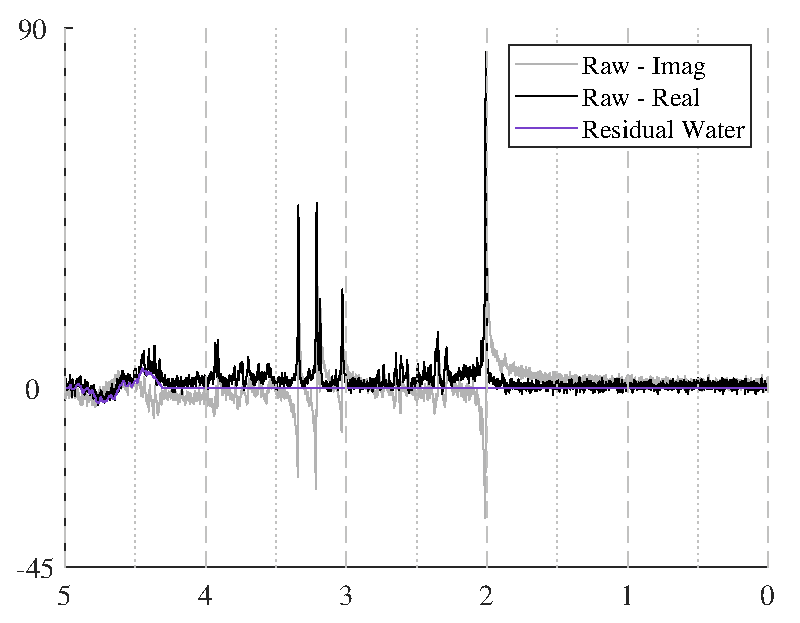
\includegraphics[width=0.93\textwidth]{images/samples_by_artifact/30ms_artifact_samples_lorentzian_1.eps}
    %     \caption{${T_2}^* \times 0.25$}
    %     \vspace{3pt}
    % \end{subfigure}&
    % \begin{subfigure}[c]{0.31\textwidth}
    %     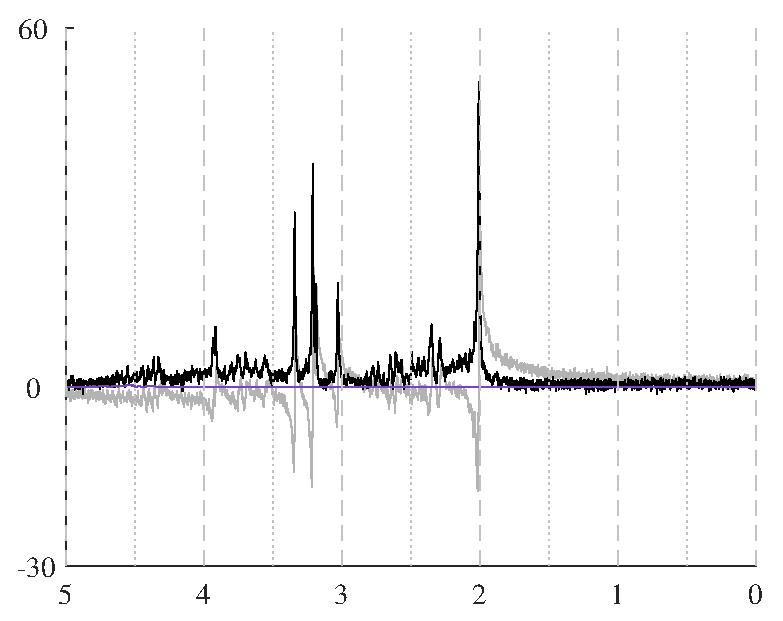
\includegraphics[width=0.93\textwidth]{images/samples_by_artifact/30ms_artifact_samples_lorentzian_2.eps}
    %     \caption{${T_2}^* \times 0.50$}
    %     \vspace{3pt}
    % \end{subfigure}&
    % \begin{subfigure}[c]{0.31\textwidth}
    %     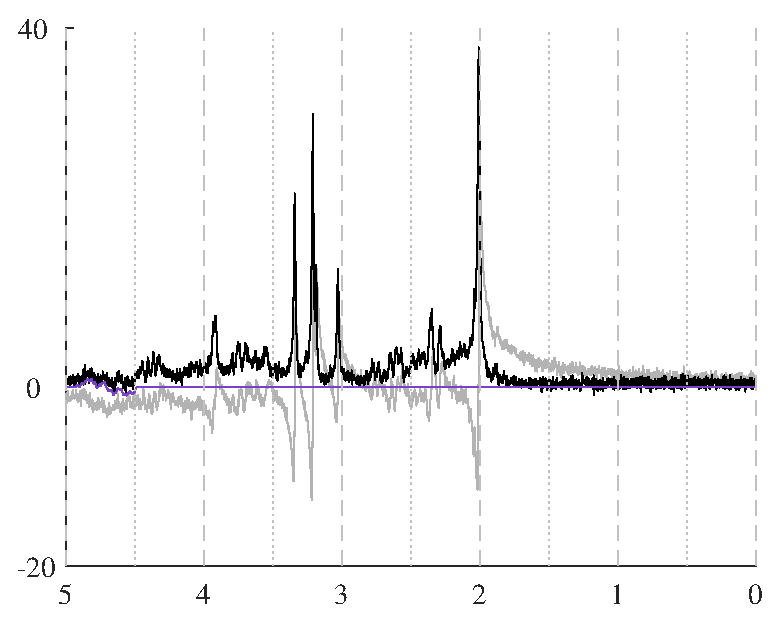
\includegraphics[width=0.93\textwidth]{images/samples_by_artifact/30ms_artifact_samples_lorentzian_3.eps}
    %     \caption{${T_2}^* \times 0.75$}
    %     \vspace{3pt}
    % \end{subfigure}\\
    % \begin{subfigure}[c]{0.31\textwidth}
    %     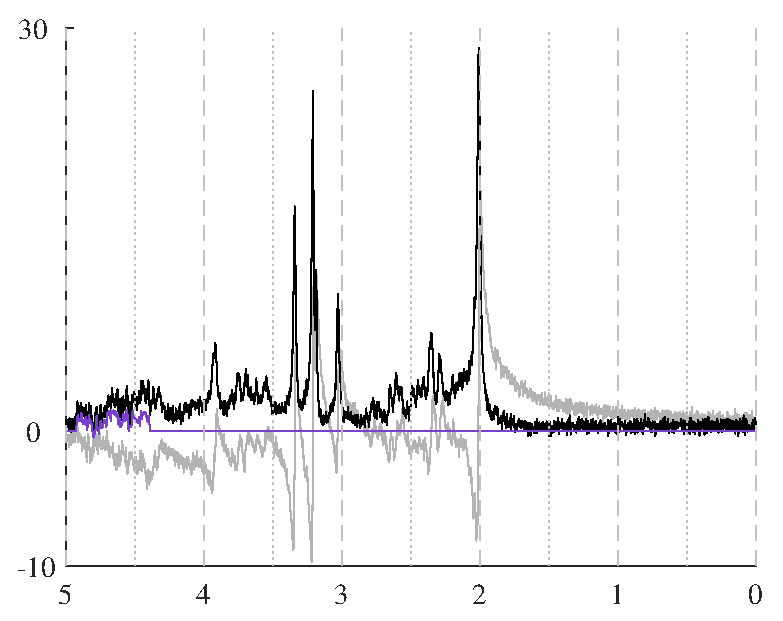
\includegraphics[width=0.93\textwidth]{images/samples_by_artifact/30ms_artifact_samples_lorentzian_4.eps}
    %     \caption{${T_2}^* \times 1.00$}
    %     \vspace{3pt}
    % \end{subfigure}&
    % \begin{subfigure}[c]{0.31\textwidth}
    %     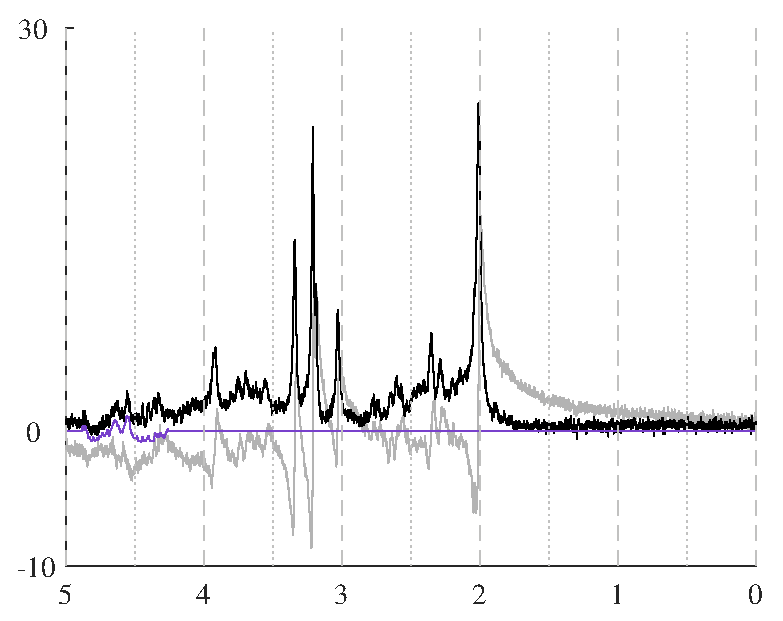
\includegraphics[width=0.93\textwidth]{images/samples_by_artifact/30ms_artifact_samples_lorentzian_5.eps}
    %     \caption{${T_2}^* \times 1.25$}
    %     \vspace{3pt}
    % \end{subfigure}&%
    % \begin{subfigure}[c]{0.31\textwidth}
    %     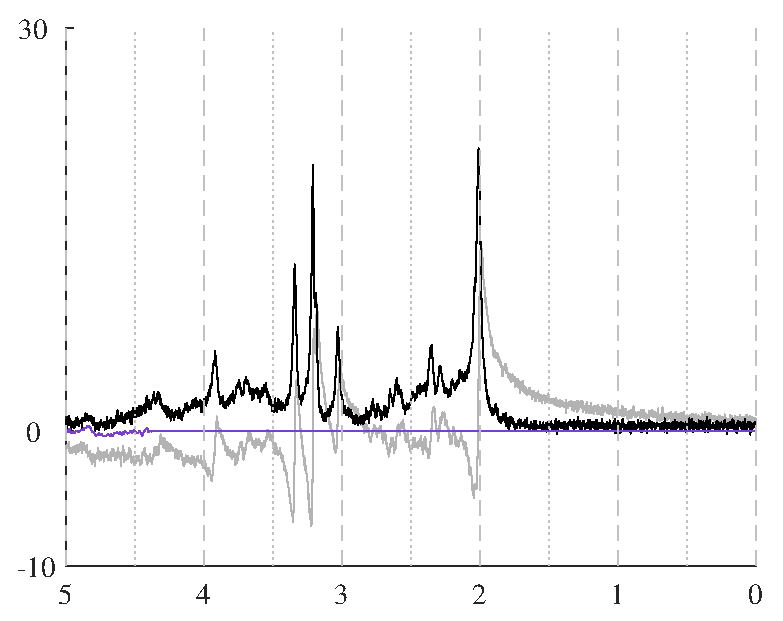
\includegraphics[width=0.93\textwidth]{images/samples_by_artifact/30ms_artifact_samples_lorentzian_6.eps}
    %     \caption{${T_2}^* \times 1.50$}
    %     \vspace{3pt}
    % \end{subfigure}\\
    % \end{tabular}
    \includegraphics[width=\textwidth,keepaspectratio]{images/compiled_figures/MRS_Sim_Figure_8_Lorentzian_Broadening_samples.png}
    \caption{${T_2}^*$ values were fixed and then scaled to represent varying magnitudes of lorentzian broadening. The spectral SNR = 15. No gaussian broadening, baselines, phase offsets, or eddy currents were included.}
    \label{fig:30ms samples lorentzians}
\end{figure}

